\chapter{Concept and Design}
\label{cha:conceptanddesign}
 
The standards presented in \autoref{cha:relatedwork} show the potential improvements that can be achieved in key components of ActiviyPub\-based social networks such as identity management, discovery, and communication. In this section, we are going to go through the different steps that are required firstly to integrate DIDs into an ActivityPub\-based social network, and finally to enable DIDComm Messaging v2 for its communication. As explained in \autoref{cha:relatedwork}, Mastodon is the social network that pioneered the use of ActivityPub on a large scale, and it is also the social network with the most active users and presence inside the Fediverse. For this reason, the ideas presented in this section and the modus operandi of the ActivityPub server are going to be scoped to the actual implementation in Mastodon.

The outline for this chapter is the following. First, individual concepts and definitions of the ActivityPub implementation are introduced and described. Then, an example of a simple use case in a contemporary ActivityPub server is going to be illustrated and analyzed in order to be able to compare it with \autoref{section:did_flow}, which presents the same use case but with the proposed concept and design that includes DID integration and DIDComm enablement, including reasons behind every decision made along with comparisons with other non\-formalized proposals.
 
\section{Definitions}
Mastodon has implemented its own ActivityPub server, and with it also its own terms to express different social network vocabulary. In order to prevent confusion or ambiguities, the used terms in this chapter are explained here. 
 
\begin{itemize}
  \item \textbf{Username}: The username in Mastodon consists of a unique local username and the domain of the instance. Ex. alice@example.com
  \item \textbf{Actor object}: In this section, the term Actor object refers solely to the ActivityPub's actor object. 
  \item \textbf{Toot}: In the user\-facing part of Mastodon, a Toot is the äquivalent of a Tweet on Twitter. This is a small status update with a 500\-character limit.
  \item \textbf{Status}: In the backend of Mastodon, the descriptor used for a Toot is a Status. Moreover, an account in Mastodon has a 1:n relationship with status.
\end{itemize}

\section{Use case}\label{section:use case}
In order to explain the current ActivityPub flow in Mastodon, let's describe what happens in the simple use case:

\emph{Alice has an account in the Mastodon instance alice\_server.com and follows Bob, who has an account in the Mastodon instance bob\_server.com. Alice sends a direct message to Bob with the text: "Hello Bob!" }

\section{Today's implementation}

% Current Flow diagram
\begin{figure}[h]
  \centering
  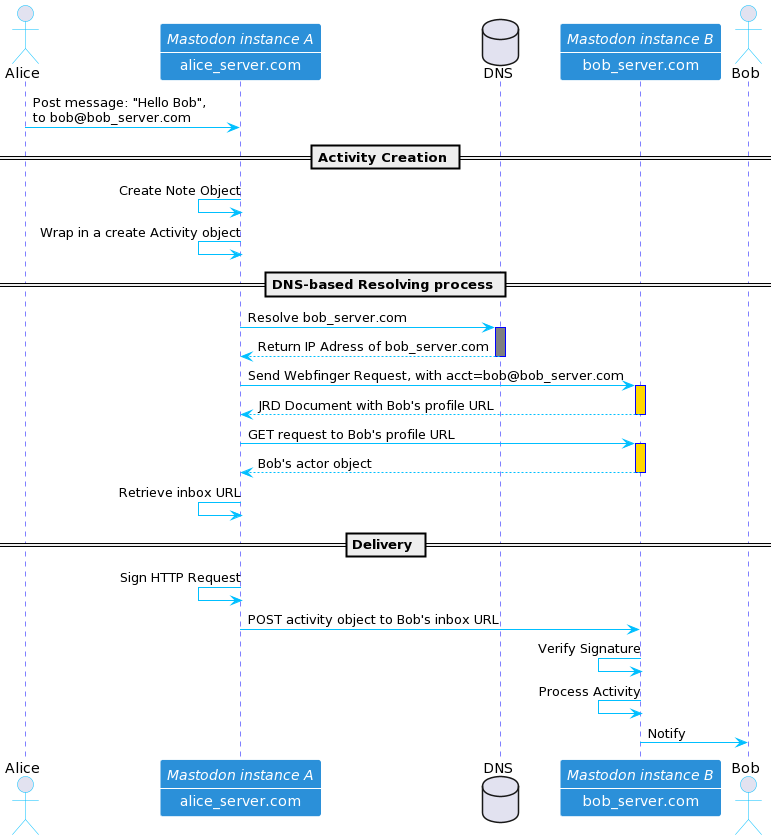
\includegraphics[width=\textwidth]{concept_and_design/normal_flow.png}
  \caption{Current flow for sending message}
  \label{fig:normal_flow}
\end{figure}

\subsection{Object creation}
The first thing that happens when Alice presses the send button is the creation of an ActivityStreams object. In this case, the object is of type \emph{Note} and will be created by the ActivityPub server inside the Mastodon instance, as shown in \ref{fig:create_note}. Then, following the ActivityPub pattern of \emph{some activity by some actor being taken on some object}, the server wraps it in an ActivityStreams \emph{Create} activity, which contains Alice as the actor. This is illustrated by \ref{fig:create_activity}. Now that the actor, the activity, and the object are well defined and wrapped, it is time to shift our focus to the recipients of this note object. 
The ActivityPub server will now look at all the fields of the ActivityStreams \emph{Audience}, which includes: to, bto, cc, bcc, and audience \cite{snell_prodromou_2017}, where all the addresses of the recipients can be retrieved. Afterward, depending on where the recipient's account lives, the ActivityPub server may take one of two options. Even though the use case explicitly dictates that Bob's account resides in a different Mastodon instance, both cases will still be explained.

% Note Object with content: 'Hello Bob'
\lstset{style=JSONStyle}
\begin{lstlisting}[language=PHP, caption=ActivityStreams note object, label=fig:create_note]
  {
    "@context": "https://www.w3.org/ns/activitystreams",
    "type": "Note",
    "to": "http://bob_server.com/users/bob",
    "attributedTo": "http://alice_server.com/users/alice",
    "content": "Hello Bob!"
  }
\end{lstlisting}

\lstset{style=JSONStyle}
\begin{lstlisting}[language=PHP, caption=ActivityStreams create activity, label=fig:create_activity]
  {
    "@context": "https://www.w3.org/ns/activitystreams",
    "type": "Create",
    "id": "https://alice_server/users/alice/statuses/634367/activity",
    "to": "http://bob_server.com/users/bob",
    "actor": "http://alice_server.com/users/alice",
    "object": {
      "type": "Note",
      "to": "http://bob_server.com/users/bob",
      "attributedTo": "http://alice_server.com/users/alice",
      "content": "Hello Bob!"
    }
  }
\end{lstlisting}


\subsection{Same\-server delivery}
If the recipient's account is on the same server, there is then no explicit discovery process. A simple query in the ActivityPub's server would find the right account and save the status within the account's statuses. 


\subsection{Discovery}
On the contrary, when the recipient's account is not on the same server, then a discovery process must be started. Discovery is the fundamental part of the federated side of Mastodon. Without it, users within different instances would not be able to interact, as the instance itself does not know where to find the actor object with all required endpoints to send or receive activities from and to external accounts. For this reason, the current way to look up other accounts is through the DNS. In the same way Email works, the domain part of the username in Mastodon points to the domain of the instance where the account lives. The purpose of the discovery in this specific use case is to find the inbox URL of Bob, which can be found in Bob's actor object. As explained in \autoref{cha:relatedwork}, Mastodon includes a series of well\-known endpoints that are used to retrieve information about the host itself, as well as resources or entities that are managed under the same host. By default, when the account is not found on the same server, a Webfinger query is performed. 
In our case, Bob's account lives inside \emph{bob\_server.com}. The request shown in \ref{fig:webfinger_request} will return a JRD Document, as shown in fig. \ref{fig:jrd_document}. Based on this document, the Mastodon instance retrieves the link with the \emph{rel: 'self'} which includes the type and the href where Bob's actor object can be retrieved. If the Webfinger request returns a 404 code, it will then try, as a fallback, using the Host\-Meta endpoint. The request and response are displayed in \ref{fig:hostmeta_request} \ref{fig:hostmeta_response}. If successful, it will then proceed to take the link template provided and try the Webfinger request once more before throwing an error. After retrieving the needed URL, a subsequent HTTP GET request to this endpoint with the specific \emph{application/activity+json} header will resolve Bob's actor object. 

\begin{lstlisting}[language=PHP, caption=Webfinger request, label=fig:webfinger_request]
  GET /.well-known/webfinger?resource=acct:bob@bob_server.com HTTP/1.1
  Host: bob_server.com
  Accept: application/ld+json
\end{lstlisting}

\lstset{style=JSONStyle}
\begin{lstlisting}[language=PHP, caption=JRD Document, label=fig:jrd_document, float=h]
  {
    "subject": "acct:bob@bob_server.com",
    "aliases": [
      "https://bob_server.com/@bob",
      "https://bob_server.com/users/bob"
    ],
    "links": [{
        "rel": "http://webfinger.net/rel/profile-page",
        "type": "text/html",
        "href": "https://bob_server.com/@bob"
      },
      {
        "rel": "self",
        "type": "application/activity+json",
        "href": "https://bob_server.com/users/bob"
      },
      {
        "rel": "http://ostatus.org/schema/1.0/subscribe",
        "template": "https://bob_server.com/authorize_interaction?uri={uri}"
      }
    ]
  }
\end{lstlisting}

\begin{lstlisting}[language=PHP, caption=Hostmeta request, label=fig:hostmeta_request, float=h]
  GET /.well-known/host-meta HTTP/1.1
  Host: bob_server.com
  Accept: application/xrd+xml
\end{lstlisting}

\lstset{style=JSONStyle}
\begin{lstlisting}[language=PHP,caption=Hostmeta response, label=fig:hostmeta_response, float=h]
  <?xml version="1.0" encoding="UTF-8"?>
  <XRD xmlns="http://docs.oasis-open.org/ns/xri/xrd-1.0">
      <Link rel="lrdd" template="https://bob_server.com/.well-known/webfinger?resource={uri}"/>
  </XRD>
\end{lstlisting}


\subsection{Delivery}
Succeeding the retrieval of Bob's actor object and therefore the needed inbox URL, the delivery can now take place. In this case, an HTTP POST request with the previously generated activity object. To provide end\-to\-end message integrity and to authenticate Alice in Bob's server, the request is signed by Alice's ActivityPub server using the HTTP Signature specification.
Finally, upon receiving the POST request to Bob's inbox URL, Bob's server verifies the validity of the signature using Alice's public key. After successful validation, it saves the Note object in Bob's statuses. 

As indicated in chapter 2, HTTP signatures are not part of the ActivityPub protocol standard. These integrity and authentication features are within the Mastodon implementation of an ActivityPub server.


\section{Proposed implementation}\label{section:did_flow}
Proposed implementation
Having seen the current flow of our use case mentioned above in a working ActivityPub\-based social network, this section will now address the first research question of this bachelor thesis. Namely, the implications of integrating DIDs to a Mastodon instance and therefore, to ActivityPub. 

\subsection{Implications of integrating DIDs}
As mentioned in the definitions section, Mastodon's full username includes the domain of the server and a locally\-unique username. This type of username accomplishes the goals of human readability and uniqueness. In addition, they are resolvable using DNS and the discovery methods previously mentioned in section \autoref{cha:relatedwork}. An ActivityPub actor object using such a username is shown in \ref{fig:alice_actor_object}.  

% Even though there are cases when very similar domains may lead to confusion and may present some security issues. Examples of this can be found simply by comparing the most used Mastodon instance “mastodon.social” with another big\\-in\-user\-count instance such as “mstdn.social”. This type of username allows the following scenarios to play out, where differences are minimal and easily missed out, such as alice@mastodon.social and alice@mstdn.social. In addition, some users have commented that when the username is too long, the domain is not longer visible. This can be exploited by malicious actors, who may open an account in a different server with the same username as their target. Clone their profile, and try to social engineer the target's followers. 

\lstset{style=JSONStyle}
\begin{lstlisting}[language=PHP, caption=Alice's actor object, label=fig:alice_actor_object, float=h]

{
	"@context": [
			"https://www.w3.org/ns/activitystreams",
			"https://w3id.org/security/v1",
	],
	"id": "http://alice_server.com/users/alice",
	"type": "Person",
	"following": "http://alice_server.com/users/alice/following",
	"followers": "http://alice_server.com/users/alice/followers",
	"inbox": "http://alice_server.com/users/alice/inbox",
	"outbox": "http://alice_server.com/users/alice/outbox",
	"featured": "http://alice_server.com/users/alice/collections/featured",
	"featuredTags": "http://alice_server.com/users/alice/collections/tags",
	"preferredUsername": "alice",
	"name": "",
	"summary": "",
	"url": "http://alice_server.com/@alice",
	"manuallyApprovesFollowers": false,
	"discoverable": false,
	"published": "2022-06-14T00:00:00Z",
}


\end{lstlisting}

The first question that needs to be addressed when approaching the integration of DIDs to Mastodon and therefore ActivityPub is, what are the implications of switching from standard mastodon usernames to DIDs. Integrating DID to ActivityPub points immediately to the actor's object. Making the switch would mean that the DID has to be included. Currently, most of the interactions of the ActivityPub server inside Mastodon require the ID attribute to resolve to the Actor's profile and thus the Actor's object. Following a simple strategy, we could simply replace the username with the DID. Thus having an ID attribute like \emph{www.alice\_server.com\/users\/did\:example\:123456789abcdefghi}.

However, there is another alternative that might work. Following the ActivityPub's specification, the ID attribute must be a publicly dereferenceable URI, whose authority belongs to the originating server \cite{lemmer-webber_tallon_guy_prodromou_2018}. As explained in \autoref{section:dids}, a DID is a URI and it is publicly dereferenceable by nature. This allows different possibilities, to which the DID can be added. Take, for example, using a stand\-alone DID as an ID attribute, to take advantage of the discoverability of DIDs. This scenario would have the following implications. If another ActivityPub Server wanted to simply get the actor's profile URL, it would require resolving the DID to its respective DID Document, adding the need to parse it and to methodically do a search until the endpoint is found and retrieved. This additionally requires that the DID Document includes the actor's profile in the services section. This modification in the DID Document will be further discussed in the Discovery section. Moreover, another option would be to add a DID URL with a query that points directly to the service endpoint that contains the actor's profile URL. Simplifying in this manner the work that the ActivityPub server must do, although still requiring a DID resolution as an intermediate step, as well as adding the service endpoint to the DID Document. Both cases are possible because ActivityPub has the URL attribute that requires the actor's profile URL in case it is not in the ID attribute \cite{lemmer-webber_tallon_guy_prodromou_2018}. Although plausible, for this Thesis we will keep a simple replacing strategy and keep the ID attribute as the profile's URL with the username replaced with the DID. 

DID URLs provide a lot of freedom of usability for DIDs. In addition to the ID, the actor's object must provide a supplementary set of URLs that point to different collections related to the Actor. These include mandatory attributes, like the outbox and the inbox, and other optional attributes such as the followers and following attributes. What if, instead of using the actual URL of these collections, we specify DID URLs that then point to the correct endpoint inside the DID Document. This example is illustrated in fig. (Activitypub actor with all DID URLs). 

This approach leads us to the question, isn't it simpler just to shift the whole actor's object endpoints directly to the DID Document? Therefore removing the need for an ActivityPub actor's object. This idea was briefly suggested by \cite{webber_sporny_2017} in a paper prepared for the 2017 Rebooting Web of Trust summit. Such an idea would look like fig. (DID Document with all ActivityPub endpoints). Furthermore, the authors went a step further and proposed cutting all dependency from the DNS by using onion websites. The authors however failed to offer an adequate explanation and consideration of the ActivityPub protocol in existing implementers. Moreover, there are some security privacy concerns regarding the use of service endpoints in the DID Document. The DID specification stipulates \emph{"revealing public information through services, such as social media accounts, personal websites, and email addresses, is discouraged"} \cite{sporny_longley_sabadello_reed_steele_2021}. DID Documents are stored in a publicly available verifiable data registry, therefore any personal information revealed here is for everyone to see. The usage of URLs in service endpoints might lead to involuntary leakage of personal information or a correlation between the URL and the DID subject. Looking at Fig(fig. DID Document with all ActivityPub endpoints), the amount of personal information displayed in the DID Document, which would not be otherwise inferable, already poses a privacy issue for the DID Subject. For this reason, in this thesis we differ from removing the actor's object from the ActivityPub protocol itself. This would also allow us to use freely all the other attributes in the actor's object to further describe its owner, such as name, preferredUsername, or summary without making this information forever public in an immutable ledger. Fig(final Actor'S object) illustrates the final design for the DID-compliant actor object. 
Regarding Mastodon, replacing the standard username with a DID does not imply huge complications. When creating a username there are some validations made to it, such as length, regex and uniqueness. All of this is contained inside the Account class, which is the object that abstracts all of a user's account. An example of the Mastodon instance that uses DIDs instead of standard usernames is illustrated in fig. (Image of Mastodon with DIDs). 


\subsection{New discovery process}
As stated in the previous section, Mastodon starts the discovery process based on the username of the user. By replacing the standard username with a DID, the current discovery flow gets disrupted, as there is no domain and thus no well-known endpoints to send discovery requests to. Nonetheless, here is where the discoverability and always resolvability of the DIDs come into play. The proposed flow of discovery takes the following steps. Firstly, the username, which now is a DID, can be resolved to its DID Document using any kind of DID resolver. An example can be the Universal Resolver from the DIF mentioned in \autoref{section:dids}. The DID Document must now contain a service section with the type ActivityPub and a URL, where the actor's object can be retrieved. This gives us 2 possibilities. On the one hand, we could add in the well-known Webfinger endpoint, which then provides us with the profile URL from the user. On the other hand, we could skip the Webfinger request and provide the profile URL directly in the DID Document. The latter looks like the most meaningful path to take. Especially when we refer to the purpose of Webfinger, which was to enable discoverability of entities represented by URIs \cite{jones_salgueiro_jones_smarr_2013}. Webfinger's purpose shares a lot of ground with the discoverable design of DIDs, nevertheless, the DID design provides a less limited structure of discovery, as it does not rely on DNS and HTTP for its functioning. For this reason, the proposed workflow will completely remove the use of the discovery protocol Webfinger used in Mastodon and include the URL of the actor's profile in the ActivityPub service section in the DID Document. 

\subsection{Enabling DIDComm Messaging}\label{section:enabling_didcomm}

Because DIDs are now implemented in our ActivityPub prototype, it is now possible to enable the DIDComm messaging protocol. Taking into account the algorithm \ref{alg:didcomm_example} shown in \autoref{section:didcomm}, it is possible to derive some requirements that DIDComm imposes:

\textbf{Key agreement}: DID Documents may present more than one verification method specified in them. A specific standard verification method is required to maintain compatibility between the parties involved. This means that the sender and the recipient must use the same set of keys for encryption and/or signing purposes to have a successful message exchange through DIDComm. The DID specification luckily provides us with a recommendation for this. The \emph{keyAgreement} verification relationship is intended to provide the keys, which allows an entity to confidentially share information with the DID-subject using encryption \cite{sporny_longley_sabadello_reed_steele_2021}. Even though it is possible to add an extra verification relationship called DIDComm or ActivityPub that works in conjunction with our previously defined ActivityPub service, we will stick to the recommendation using the \emph{keyAgreement} key for our proposal.

\textbf{Access to private key}: The ActivityPub server requires access to the private key of the selected verification method. This of course imposes risks, as the private key is no longer in the user's control. The administrator of the Mastodon instance would have access to the plain-text private key, and some security countermeasures like key rotation would not be able to counter this. Furthermore, the ActivityPub server must be able to support the keys and the cryptographic algorithms, which the JWA includes. This means having any kind of library that can parse them and perform encryption as well as decryption with them.

\textbf{Access to DID-Resolver}: The ActivityPub server must have access to a DID-Resolver to be able to retrieve DID Documents. Especially in cases where an incoming message has been signed, and the signature needs to be verified using a specific public key. This requires extending the Mastodon server by adding possibly a service class that performs calls to a DID-resolver and parses the returned DID Document to process the information in it. 

\subsubsection{ActivityPub as DIDComm payload}

As part of this proposal, we do not want to do further changes to the ActivityPub protocol itself. However, extending it and removing the dependency on the HTTP protocol for its communication is still intended. Therefore, encapsulation rather than modification of ActivityPub within DIDComm allows for a modular approach that keeps both protocols independent from each other. DIDComm presented 3 different kinds of message structures, namely plain text (JWM), signed (JWS) and encrypted messages (JWE). The following sections present how the encapsulation, as well as signing and encryption processes, work in this proposal.

\textbf{ActivityPub as JWM}: Let's take our previous example of an ActivityStreams object where Alice sends a message to Bob. The simplest way to keep a modular approach is by using the ActivityStream object as a payload for our JWM, which would look like fig. (JWM with activity). As explained in chapter 2, the JWM specification defines a series of attributes that provide a starting point for the use of JWMs. Not all of these are mandatory and can thus be modified depending on the use being given to them. This gives us a lot of room to think about what is necessary and what is not. As seen in fig. (JWM with activity), redundancy can be found in each level of the JSON object. For example, the sender and recipient are defined in each layer. In the end, the Activity is the only object that will be processed, therefore, the JWM does not necessarily need any extra information, because the Activity has already all the necessary information. Furthermore, even if we wanted to use the routing mechanism of DIDComm, the attributes From and To in the JWM would only be necessary in cases where we want to send plain text messages. In addition, in almost every case the message is being sent to a specific URL, like the inbox of another user. So the receiver server will always know to whom the Activity was directed. This leaves us with a JWM structure with the attributes id and type. The requiredness of these two differs from the JWM specification and DIDComm. Nonetheless, we will stick to DIDComm and keep these two attributes compulsory. The type should be a message type URI, therefore we will use the ActivityStreams schema URI, and for the ID, we will reuse the status ID. The result is shown by figure \ref{fig:jwm_example}

\lstset{style=JSONStyle}
\begin{lstlisting}[language=PHP, caption=JWM example, label=fig:jwm_example, float=h]
  {
    "id": "https://alice_server/users/did:example:alice/statuses/634367/activity",
    "type": "https://www.w3.org/ns/activitystreams",
    "body": {
      "@context": "https://www.w3.org/ns/activitystreams",
      "type": "Create",
      "id": "https://alice_server/users/did:example:alice/statuses/634367/activity",
      "actor": "https://alice_server.com/users/did:example:alice",
      "to": [ 
            "https://bob_server.com/users/did:example:bob"
        ],
      "object": {
        "type": "Note",
        "to": [ 
            "https://bob_server.com/users/did:example:bob"
        ],
        "attributedTo": "https://alice_server.com/users/did:example:alice",
        "content": "Hello Adrian!"
      }
    }
  }
\end{lstlisting}



The final flow for our use case mention in\ref{section:use case} is illustrated in figure \ref{fig:did_flow}

% Proposed Flow diagram
\begin{figure}[h]
  \centering
  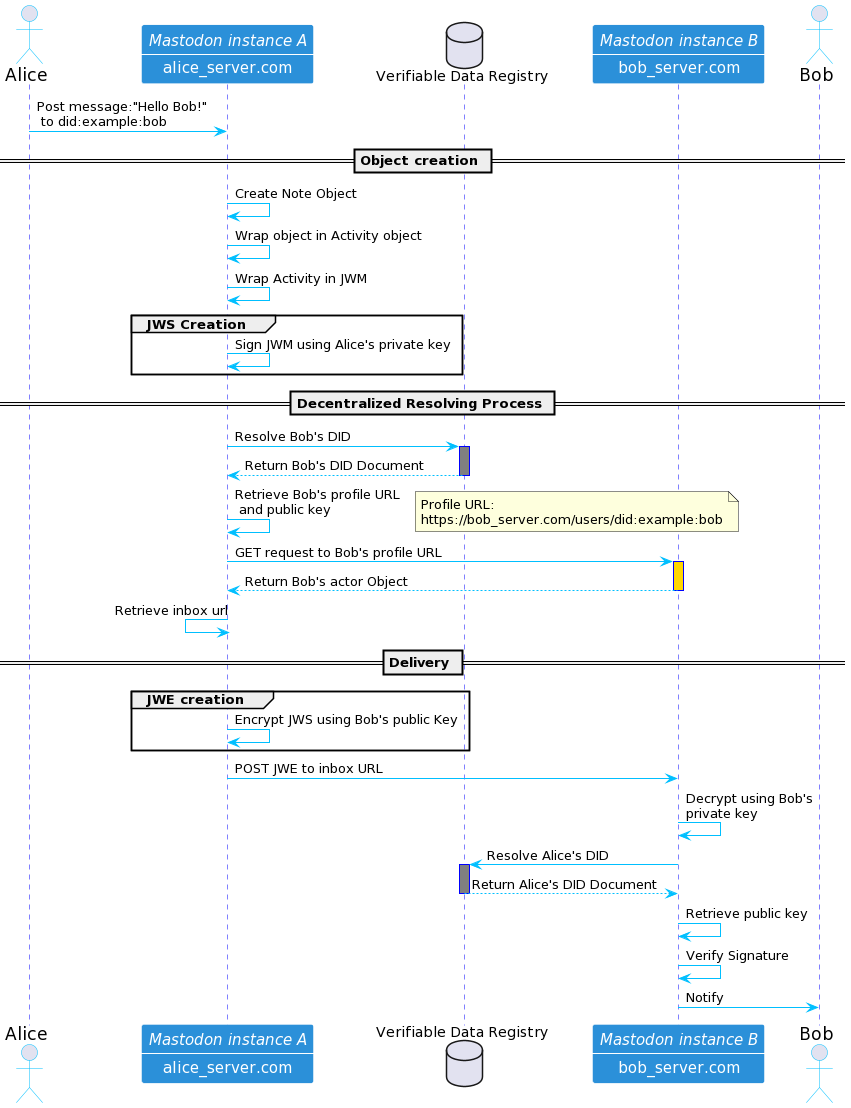
\includegraphics[width=\textwidth]{concept_and_design/did_flow.png}
  \caption{DID and DIDComm flow for use case}
  \label{fig:did_flow}
\end{figure}

% @startuml
% actor Alice as a
% participant Alice_Server as as
% database VDR
% participant Bob_Server as bs
% actor Bob as b

% a->as: Message to Bob: "Hello Bob!"
% as<-as: Create Note Object
% as<-as: Wrap object in Activity
% as<-as: Sign using Alice's private key

% == Discovery ==
% as->VDR ++ #gray: Resolve Bob's DID
% VDR-->as --: Bob's DID Document
% as<-as: Retrieve service endpoint \n url and public_key 
% as<-as: Encrypt using\nBob's public Key

% as->bs ++ #gold: GET service endpoint url
% bs-->as --: Bob's actor Object
% as<-as: Retrieve inbox url

% == Delivery ==
% as->bs: POST encrypted message

% bs<-bs: Decrypt using Bob's\nprivate key
% bs->VDR ++ #gray: Resolve Alice's DID
% VDR-->bs --: Alice's DID Document

% bs<-bs: Retrieve public_key 
% bs<-bs: Verify Signature

% bs->b: Notify
% b<-b: Read Message

% @enduml


% @startuml
% actor Alice as a
% participant Alice_server as as
% database DNS
% participant Bob_server as bs
% actor Bob as b

% a->as: Post message: "Hello Bob!"
% as<-as: Create Note Object
% as<-as: Wrap object in Activity

% == Discovery ==


% as->DNS ++ #gray: Resolve Bob's server domain
% DNS-->as --: Return IP Adress of bob-server.com

% as->bs ++ #gold: Send Webfinger Request
% bs-->as --: JRD Document describing Bob
% as<-as: Retrieve Bob's \nprofile url

% as->bs ++ #gold: GET user profile url
% bs-->as --: Bob's actor object
% as<-as: Retrieve inbox \nurl

% == Delivery ==
% as->bs: POST message to Bob's inbox url

% bs->b: Notify

% b<-b: Read message

% @enduml